\documentclass{uninove-ppgi} %courier ou times

\begin{document}
\lstset{
    language=xml,
    tabsize=3,
    frame=shadowbox,
    rulesepcolor=\color{gray},
    xleftmargin=20pt,
    framexleftmargin=15pt,
    keywordstyle=\color{blue}\bf,
    commentstyle=\color{OliveGreen},
    stringstyle=\color{red},
    numbers=left,
    numberstyle=\tiny,
    numbersep=5pt,
    breaklines=true,
    showstringspaces=false,
    basicstyle=\footnotesize,
    emph={food,name,price},emphstyle={\color{magenta}}
}

% Posiciona o logo da Uni9 no topo

\includegraphics[height=1.5cm]{uninove-logo}

% parametros de capa e folha de rosto (é necessário configurar todos)
\Universidade{UNIVERSIDADE NOVE DE JULHO - UNINOVE}

\Autor{EXCLUÍDOS OS DADOS SOBRE OS AUTORES EM ATENDIMENTO A LGPD - LEI GERAL DE PROTEÇÃO DE DADOS}

\Titulo{Digital Jungle Quest}

% Inserir o nome do projeto no formato que está abaixo (Olhe o nome da disciplina na central do aluno)
\Tipoprojeto{PROJETO EM EMPREENDEDORISMO}

% Informe qual o curso: Bacharel ou Tecnólogo + curso
\Curso{Tecnólogo em Análise e Desenvolvimento de Sistemas}

% NÃO ALTERAR
\Orientador{Edson Melo de Souza, Dr.}

% Inserir o ano correspondente
\Ano{2024}

% gera a capa automaticamente
\capa

% gera folha de rosto automaticamente
\folharosto

% ##################### Início dos elementos pré-textuais ############################

% Resumo (Obrigatório)
% !TEX root = ..\main.tex

\PalavrasChave{estudantes, profissionais, aprendizagem, educação, desenvolvimento, resultados.}
\centeredchapterstyle
\begin{resumo}
   \noindent\textbf{Contexto}: A Lost in the Digital Jungle, startup pioneira fundada em 2020, tem como missão principal fornecer uma plataforma de aprendizagem gamificada. \textbf{Objetivo}: é capacitar estudantes universitários e profissionais para enfrentar os desafios do mundo digital. \textbf{Método}: de aprendizagem gamificada para alcançar seus objetivos. Esse método se baseia nos seguintes princípios: elementos de jogos, desafios, recompensas e competição.\textbf{Resultados}: apesar de ser uma empresa relativamente nova, já obteve resultados expressivos em seu curto período de existência. Entre os principais resultados da empresa, podemos destacar: crescimento da base de alunos, altos índices de satisfação e reconhecimento da indústria. \textbf{Conclusão}: A Lost in the Digital Jungle se destaca como uma empresa inovadora e promissora no cenário da educação tecnológica. Através de sua plataforma de aprendizagem gamificada, a empresa oferece uma solução eficaz e engaging para o desenvolvimento de habilidades digitais em estudantes universitários e profissionais.
\end{resumo}

% Abstract (Obrigatório) - resumo em inglês
% !TEX root = ..\main.tex

\KeyWords{students, professionals, learning, education, development, results.}
\centeredchapterstyle
\begin{abstract}
   \noindent\textbf{Context}: Lost in the Digital Jungle, a pioneering startup founded in 2020, has as its main mission to provide a gamified learning platform. \textbf{Objective}: is to train university students and professionals to face the challenges of the digital world. \textbf{Method}: gamified learning to achieve your goals. This method is based on the following principles: game elements, challenges, rewards and competition.\textbf{Results}: despite being a relatively new company, it has already achieved significant results in its short period of existence. Among the company's main results, we can highlight: growth in the student base, high levels of satisfaction and industry recognition. \textbf{Conclusion}: Lost in the Digital Jungle stands out as an innovative and promising company in the technological education scene. Through its gamified learning platform, the company offers an effective and engaging solution for developing digital skills in university students and professionals.
\end{abstract}


% Sumário (Obrigatório)
\begingroup
\makeatletter \let\ps@plain\ps@empty \makeatother 
\tableofcontents
\
\endgroup
\thispagestyle{empty}

% Lista de figuras
\renewcommand*\listfigurename{Lista de Ilustrações}
\listoffigures
\thispagestyle{empty}

\listoftables
\thispagestyle{empty}


\regularchapterstyle

% ############### Início dos Capítulos (Obrigatório ) #################

% Introdução
\renewcommand{\thefigure}{\arabic{figure}}

\chapter{Introdução}
\label{ch:introducao}
\begin{resumocapitulo}
Digital Jungle Quest:
Fundada em 2020, a Digital Jungle Quest é uma startup inovadora que oferece uma plataforma de aprendizagem gamificada para auxiliar estudantes universitários e profissionais a aprimorarem suas habilidades digitais.
 \textbf{citação} (\textit{arquivo refs.bib}), \textbf{tabelas}, \textbf{quadros}, \textbf{equações} e \textbf{algoritmos}. Para ter acesso a documentação diretamente na biblioteca da Uninove, \href{http://docs.uninove.br/arte/pdfs/Manual_de_Trabalhos_Academicos_ABNT_UNINOVE.pdf}{clique aqui.}
\end{resumocapitulo}

\chapter{Objetivos}
\label{ch:Objetivos}
Na Digital Jungle Quest, nosso objetivo é ser a bússola que guia os indivíduos em sua jornada pelo ambiente virtual. Comprometemo-nos a fornecer as ferramentas inovadoras, o conhecimento de ponta e o apoio personalizado necessários para que cada aluno possa alcançar seus objetivos educacionais e profissionais. Acreditamos que, com a orientação e os recursos adequados, todos podem concluir seus estudos com confiança e proficiência, preparados para enfrentar os desafios e aproveitar as oportunidades do mundo digital.

\chapter{Sobre Nós}
\label{ch:Sobre Nos}
Sobre Nós
A Digital Jungle Quest nasceu em 2020 com a visão de revolucionar a educação digital. Somos uma startup dedicada a transformar a maneira como jovens alunos e profissionais da área de tecnologia aprendem e desenvolvem suas habilidades. Utilizando uma abordagem gamificada inovadora, nossa plataforma oferece uma experiência de aprendizado envolvente e motivadora, que combina tecnologia de ponta com práticas pedagógicas eficazes.

\begin{figure}
    \centering
    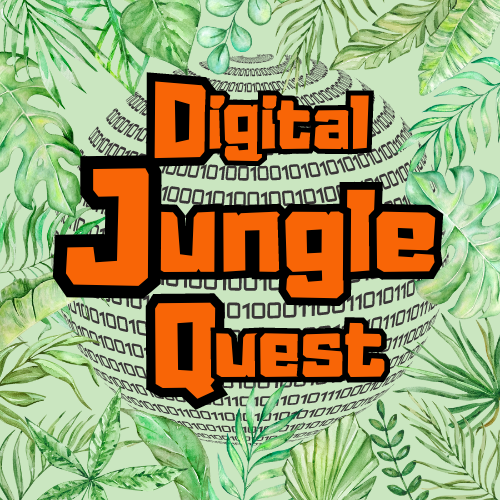
\includegraphics[width=0.75\linewidth]{figuras/DigitalJungleQuestLOGO.png}
    \caption{Digital Jungle Quest LOGO}
    \label{fig:enter-label}
\end{figure}

\chapter{Ideação}
\label{ch:Ideação}
Nossa missão é capacitar a próxima geração de profissionais de tecnologia através de uma educação acessível, interativa e estimulante. Acreditamos que o aprendizado deve ser uma aventura emocionante, repleta de desafios e recompensas que incentivam o progresso contínuo e a aquisição de competências essenciais para o futuro.

Nossa Visão, visualizamos um mundo onde o aprendizado digital é sinônimo de diversão e eficácia. Através da gamificação, queremos criar um ambiente onde os alunos não apenas adquirem conhecimento, mas também desenvolvem habilidades práticas e aplicáveis, essenciais para a carreira na área tecnológica. Nosso objetivo é ser a plataforma líder em educação digital gamificada, reconhecida pela inovação e pelo impacto positivo na formação de profissionais competentes e confiantes.

Nossos Valores

Inovação:
Estamos comprometidos em oferecer soluções educacionais inovadoras que aproveitem as últimas tecnologias e tendências pedagógicas.

Engajamento:
Criamos experiências de aprendizado que mantêm os alunos motivados e engajados, promovendo a retenção e a aplicação prática do conhecimento.

Acessibilidade:
Acreditamos que a educação de qualidade deve ser acessível a todos, independentemente de sua localização ou circunstâncias financeiras.

Excelência:
Buscamos constantemente a excelência em tudo o que fazemos, desde o desenvolvimento de conteúdo até o suporte ao cliente.

Colaboração:
Valorizamos a colaboração e o feedback dos nossos usuários para melhorar continuamente a nossa plataforma e oferecer uma experiência educativa de alta qualidade.

\chapter{Validação da Ideia}
\label{ch:Validacao_da_Ideia}
Na Digital Jungle Quest, acreditamos no poder da inovação e da gamificação para transformar a educação digital. Desde a nossa fundação em 2020, nosso objetivo tem sido criar uma plataforma de aprendizado envolvente e eficaz, destinada a jovens estudantes e profissionais da área de tecnologia. Aqui está como validamos nossa ideia para garantir que estamos atendendo às necessidades de nossos usuários:

Pesquisa de Mercado Inicial
Para entender as necessidades e desafios de nossos potenciais usuários, conduzimos uma pesquisa de mercado abrangente. Realizamos entrevistas detalhadas com estudantes e profissionais de tecnologia para identificar suas dificuldades e preferências no aprendizado digital. Também distribuímos questionários online em fóruns de tecnologia e redes sociais para coletar dados quantitativos. Essa fase inicial foi crucial para identificar o alto interesse por uma abordagem gamificada no aprendizado de habilidades digitais.

Desenvolvimento de um MVP
Com os insights da pesquisa de mercado, desenvolvemos um MVP (Produto Mínimo Viável) que incorporou as funcionalidades essenciais da nossa plataforma. Criamos um protótipo de baixa fidelidade para visualizar a interface e as mecânicas de jogo. Implementamos cursos interativos, quizzes gamificados e um sistema de pontos e recompensas. Este MVP foi lançado para um grupo seleto de usuários em um teste piloto, permitindo-nos obter feedback valioso sobre a usabilidade e o engajamento.

Análise de Dados e Iteração
A análise dos dados de uso e o feedback direto dos usuários do teste piloto foram fundamentais para aprimorar nossa plataforma. Utilizamos ferramentas de análise para monitorar o comportamento dos usuários e identificar áreas de melhoria. Realizamos entrevistas detalhadas e questionários de satisfação para coletar feedback qualitativo. Com base nisso, fizemos ajustes significativos na interface, nas funcionalidades gamificadas e na experiência geral do usuário.

Validação com um Público Maior
Para validar a escalabilidade da nossa plataforma, expandimos o teste para um público maior e mais diversificado. Lançamos um beta público, colaborando com instituições educacionais e empresas de tecnologia para promover a Digital Jungle Quest. Continuamos a coletar feedback contínuo e a realizar atualizações baseadas nas sugestões dos usuários. Essa fase nos permitiu confirmar a viabilidade da plataforma em uma escala maior e identificar oportunidades de crescimento.

Ajustes Finais e Lançamento Oficial
Com os dados e feedback coletados, implementamos as melhorias finais necessárias para preparar a Digital Jungle Quest para o lançamento oficial. Desenvolvemos uma estratégia de marketing robusta para destacar os diferenciais da nossa plataforma gamificada. Estabelecemos um sistema de suporte ao cliente eficiente para atender às necessidades dos novos usuários. Em 2021, lançamos oficialmente a Digital Jungle Quest, proporcionando uma experiência de aprendizado digital inovadora e envolvente.

% Base Teórica
\chapter{Fundamentação Teórica}
\label{ch:Fundamentação_Teorica}
	\begin{resumocapitulo}
		No cenário contemporâneo, a demanda por profissionais qualificados em habilidades digitais é exponencialmente crescente. Nesse contexto, a Digital Jungle Quest emerge como uma instituição de ensino pioneira, oferecendo uma plataforma de aprendizagem gamificada destinada a auxiliar estudantes universitários e profissionais na ampliação e aprimoramento de suas competências digitais. Através de uma abordagem interativa e imersiva, a Digital Jungle Quest proporciona uma experiência educacional única, fundamentada em uma grade curricular abrangente e atualizada, que engloba diversos aspectos essenciais das tecnologias digitais contemporâneas.
	\end{resumocapitulo}

	\section{Fundamentação Teórica da Grade Curricular da Digital Jungle Quest}

\begin{figure}
\centering
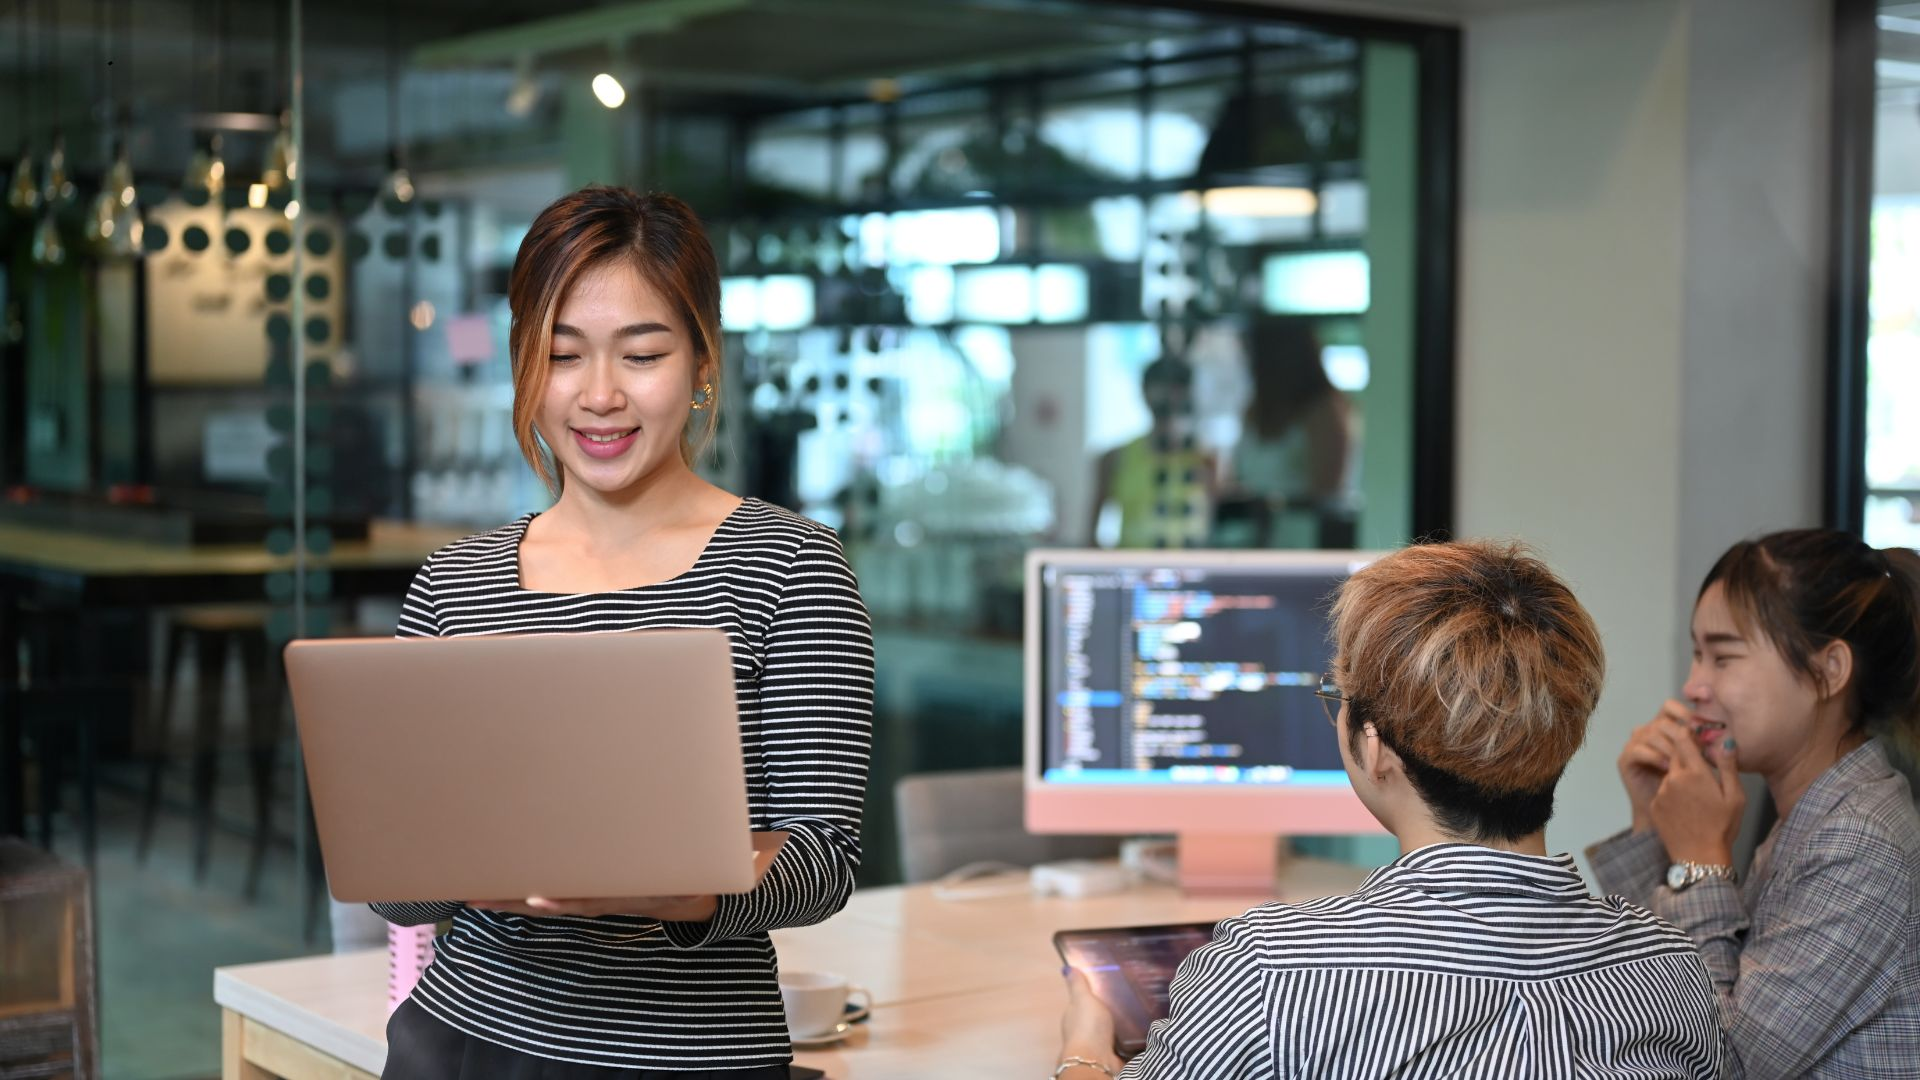
\includegraphics[width=0.75\linewidth]{figuras/fundamentação.jpg}
\caption{Fundamentação Teórica}
\end{figure}

Fundamentação Teórica

A fundamentação teórica da Digital Jungle Quest é embasada em uma seleção criteriosa de materiais de referência, cuidadosamente escolhidos para fornecer uma base sólida e abrangente aos estudantes em sua jornada de aprendizado. A seguir, destacamos algumas das disciplinas fundamentais oferecidas pela instituição, juntamente com os materiais base utilizados para cada uma delas.

Programação Front-End: HTML, CSS e JavaScript

A programação front-end é um pilar fundamental no desenvolvimento de aplicações web modernas. Para proporcionar aos estudantes uma compreensão abrangente dos elementos essenciais do front-end, a Digital Jungle Quest incorpora uma variedade de recursos de alta qualidade em sua abordagem pedagógica.

HTML: A base estrutural de qualquer página web, o HTML é ensinado através de recursos como o artigo "HTML5: A Vocabulary and Associated APIs for HTML and XHTML" pelo World Wide Web Consortium (W3C), que detalha a especificação oficial do HTML5. Complementando este conhecimento, o livro "HTML and CSS: Design and Build Websites" de Jon Duckett oferece uma introdução abrangente aos fundamentos do HTML e CSS, consolidando os princípios básicos da linguagem.

CSS (Cascading Style Sheets): Para aprofundar o entendimento de CSS, são utilizados recursos como o livro "CSS: The Definitive Guide" por Eric A. Meyer e Estelle Weyl, que abrange todos os aspectos do CSS, incluindo layouts e animações. Além disso, a publicação "CSS3: Visual QuickStart Guide" de Jason Cranford Teague explora as novas funcionalidades do CSS3, garantindo uma compreensão abrangente das capacidades mais recentes da linguagem.

JavaScript: Considerado uma das linguagens de programação mais importantes no desenvolvimento web, o JavaScript é ensinado através de obras como "JavaScript: The Good Parts" de Douglas Crockford, que oferece insights sobre as melhores práticas e abordagens eficientes na linguagem. Além disso, "Eloquent JavaScript: A Modern Introduction to Programming" de Marijn Haverbeke fornece uma introdução moderna e acessível aos conceitos fundamentais do JavaScript, preparando os estudantes para enfrentar os desafios da programação front-end com confiança e competência.

IoT (Internet das Coisas) e Arquitetura de Computadores

Além das disciplinas tradicionais de programação web, a Digital Jungle Quest também oferece uma visão abrangente e prática de tópicos avançados, como IoT e Arquitetura de Computadores.

IoT: Para a disciplina de IoT, é adotado o livro "Internet of Things: A Hands-On Approach" de Arshdeep Bahga e Vijay Madisetti, que oferece uma introdução prática e baseada em projetos ao desenvolvimento de soluções IoT. Através deste recurso, os estudantes são capacitados a compreender os princípios fundamentais por trás da Internet das Coisas e a aplicar seus conhecimentos na criação de soluções inovadoras e funcionalidades conectadas.

Arquitetura de Computadores: A compreensão da arquitetura de computadores é essencial para qualquer profissional de tecnologia da informação. Para essa disciplina, é utilizado o livro "Computer Organization and Design: The Hardware/Software Interface" de David A. Patterson e John L. Hennessy, uma obra clássica que aborda os princípios fundamentais da arquitetura de computadores de forma abrangente e acessível. Através deste recurso, os estudantes desenvolvem uma compreensão sólida dos componentes essenciais de um sistema computacional e de sua interação com o software subjacente.

Considerações Finais

Em suma, a Digital Jungle Quest representa uma abordagem inovadora e abrangente no ensino de habilidades digitais, oferecendo uma plataforma de aprendizagem gamificada que combina teoria e prática de forma integrada e envolvente. Através de uma grade curricular cuidadosamente elaborada e de uma seleção criteriosa de materiais de referência, a instituição prepara os estudantes para enfrentar os desafios do mundo digital com confiança, competência e criatividade.

% Metodologia
\chapter{Metodologia}
\label{ch:identificador}
\begin{resumocapitulo}
    A metodologia da Digital Jungle Quest combina gamificação e aprendizado ativo, oferecendo uma experiência de ensino envolvente e personalizada para programadores e estudantes de tecnologia. Nosso currículo modular permite uma progressão individualizada, focando em hard skills, como linguagens de programação e frameworks, e soft skills, como comunicação e trabalho em equipe. A avaliação contínua e o feedback bidirecional garantem a melhoria constante, enquanto a mentoria individual e a comunidade de aprendizado proporcionam suporte contínuo. Utilizamos análises de dados para aprimorar nosso currículo e estamos comprometidos com a inovação contínua, preparando os alunos para os desafios do mercado de trabalho tecnológico.
\end{resumocapitulo}

\begin{figure}
    \centering
    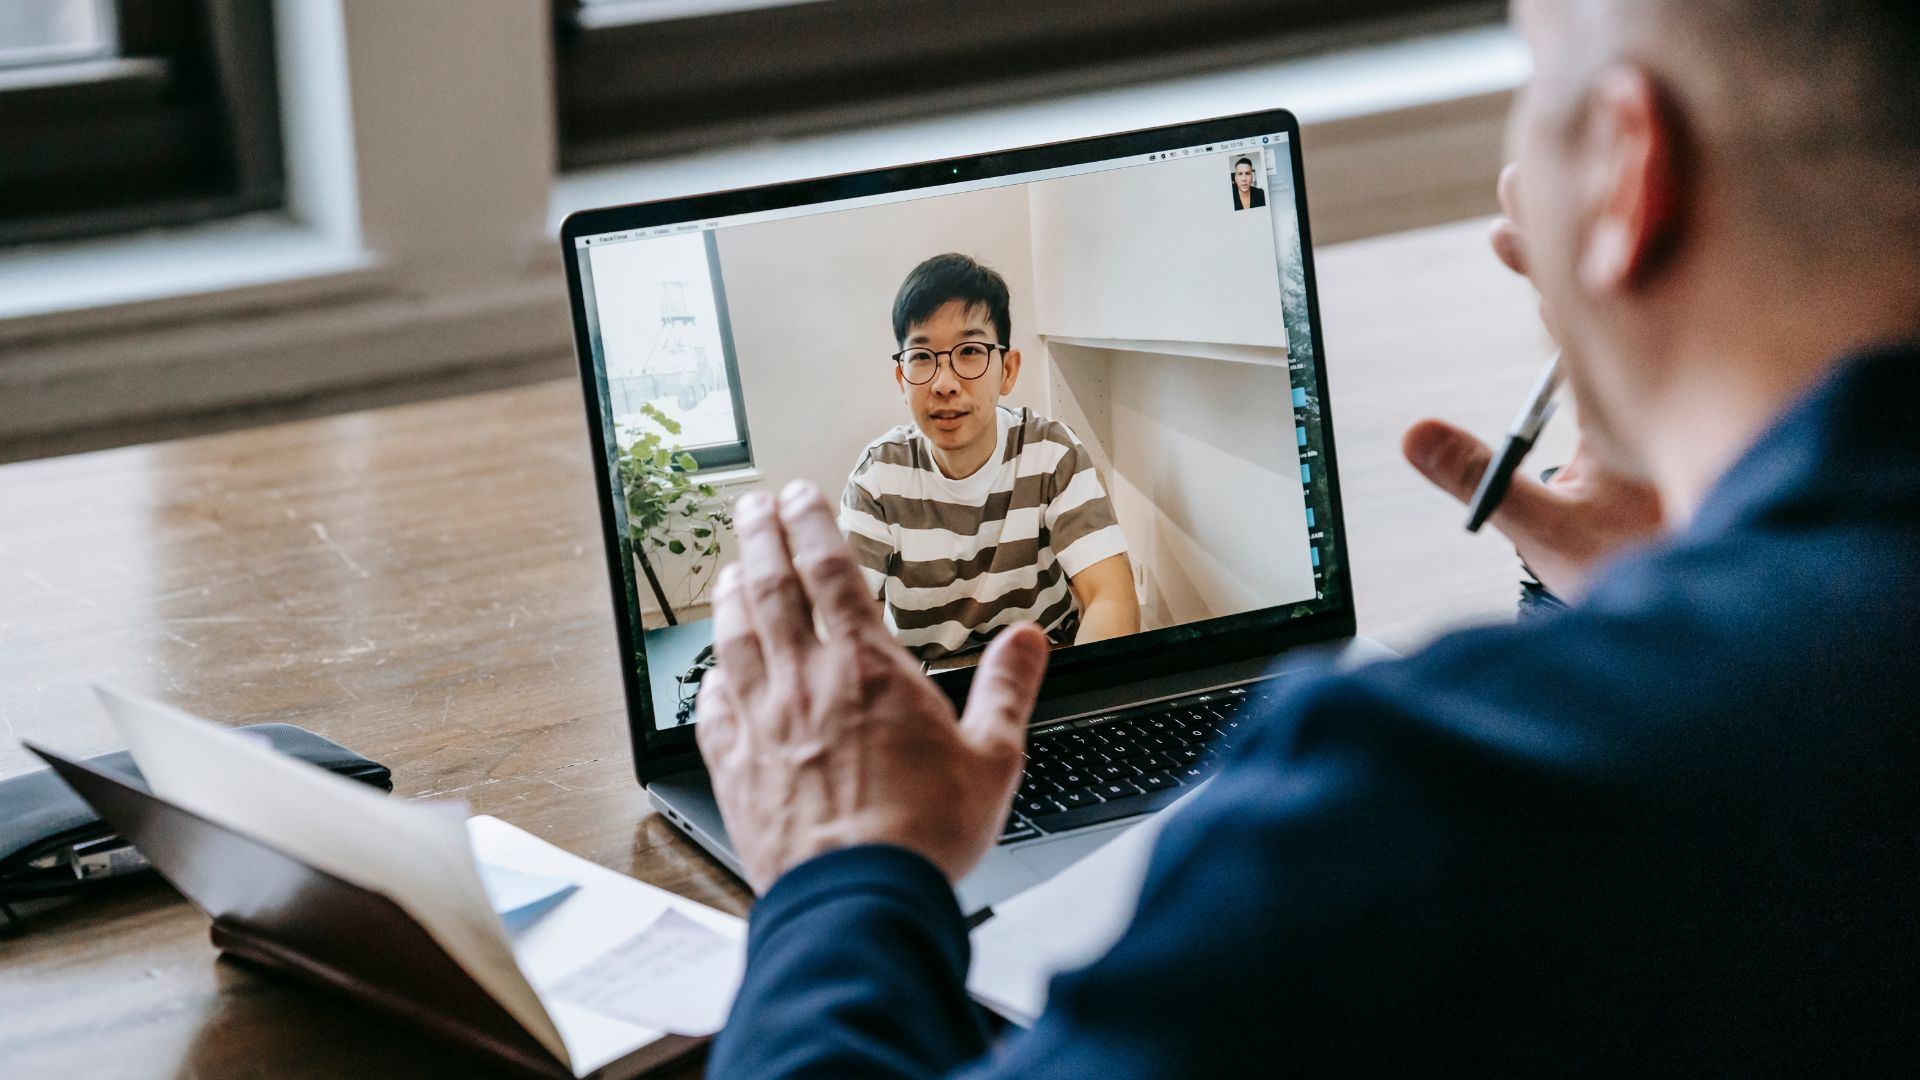
\includegraphics[width=0.75\linewidth]{figuras/metodologia.jpg}
    \caption{metodologia}
    \label{fig:enter-label}
\end{figure}

\section{Visão Geral}
A Digital Jungle Quest adota uma metodologia inovadora e eficaz para proporcionar uma experiência de aprendizado envolvente e contínua para programadores e estudantes de tecnologia. Nosso objetivo é formar profissionais altamente capacitados, prontos para enfrentar os desafios do mercado de trabalho moderno. A seguir, detalhamos os principais pilares da nossa metodologia institucional.

\section{Abordagem de Ensino}
\label{sec:Abordagem de Ensino}
Gamificação:
Na Digital Jungle Quest, acreditamos que o aprendizado deve ser uma aventura estimulante. Implementamos um sistema de gamificação robusto onde os alunos acumulam pontos e recompensas à medida que completam tarefas, quizzes e projetos. Os alunos são incentivados por rankings semanais e mensais, promovendo uma competição saudável que estimula o progresso contínuo. Desafios temáticos regulares e missões práticas integram diversos conceitos aprendidos, fortalecendo a aplicação do conhecimento em situações reais.

\section{Aprendizado Ativo}
\label{sec:Aprendizado Ativo}
Nosso currículo é centrado em projetos práticos que exigem a aplicação direta dos conhecimentos adquiridos. Os alunos participam de workshops e hackathons regulares, enfrentando problemas do mundo real com a orientação de mentores experientes. Essa abordagem garante que nossos alunos não apenas entendam a teoria, mas também dominem as habilidades práticas necessárias para suas carreiras.

\section{Desenvolvimento de Habilidades}
\label{sec:Desenvolvimento de Habilidades}

Hard Skills:\\
Na Digital Jungle Quest, nossa oferta educativa abrange uma ampla gama de linguagens de programação, linguagens front-end, desenvolvimento IoT, entre outras. Além disso, fornecemos instrução detalhada em frameworks, bibliotecas e ferramentas de desenvolvimento contemporâneas, preparando os alunos para o ambiente tecnológico dinâmico e exigente.

Soft Skills:\\
Valorizamos o desenvolvimento integral dos nossos alunos, por isso incluímos treinamentos focados em habilidades de comunicação, trabalho em equipe e gerenciamento de tempo. Projetos colaborativos e metodologias ágeis são utilizados para simular ambientes de trabalho reais, promovendo habilidades interpessoais essenciais.

\section{Inovação Contínua}
\label{sec:Inovação Contínua}
Estamos comprometidos com a inovação contínua. Atualizamos regularmente nossos conteúdos para incluir as mais recentes tecnologias e práticas do setor e desenvolvemos novas funcionalidades na plataforma para melhorar a experiência de aprendizado dos nossos alunos.

A metodologia da Digital Jungle Quest visa não apenas equipar os alunos com habilidades técnicas, mas também prepará-los para o mercado de trabalho, promovendo um aprendizado contínuo e uma mentalidade de crescimento. Nossa abordagem integral e inovadora garante que cada aluno esteja preparado para enfrentar e superar os desafios do mundo da tecnologia.

\section{Análise dos Resultados}
\label{ch:resultados}
A Digital Jungle Quest, fundada em 2020, tem demonstrado um crescimento impressionante desde sua criação. Com uma abordagem inovadora de marketing e estratégias de divulgação direcionadas a um público jovem e moderno, utilizamos plataformas como TikTok e Instagram para alcançar e engajar nossos potenciais alunos. No primeiro ano, contamos com 20 alunos e uma equipe de 10 colaboradores dedicados.

Ao longo dos anos, nosso compromisso com a qualidade educacional e o desenvolvimento contínuo de nossos programas resultou em um aumento significativo no número de alunos e profissionais. Atualmente, temos 260 alunos em curso e uma equipe ampliada de 30 profissionais especializados atuando em diversas áreas da Digital Jungle Quest.

Este crescimento representa um aumento gradual médio de aproximadamente 60 alunos por ano, evidenciando a eficácia de nossas estratégias e a crescente demanda por educação tecnológica de qualidade. Estamos orgulhosos dos resultados alcançados e continuamos comprometidos em proporcionar uma experiência de aprendizagem excepcional para nossos alunos, preparando-os para enfrentar os desafios do ambiente tecnológico dinâmico e exigente.

Com nossa metodologia centrada no desenvolvimento integral, incluindo treinamentos em soft skills e a aplicação de metodologias ágeis, garantimos que nossos alunos não apenas adquiram conhecimentos técnicos, mas também habilidades interpessoais essenciais para o mercado de trabalho. A Digital Jungle Quest continua a se expandir e a inovar, consolidando-se como uma referência em educação tecnológica.




% Resultado
\chapter{Análise dos Resultados}
\label{ch:resultados}
A Digital Jungle Quest, fundada em 2020, tem demonstrado um crescimento impressionante desde sua criação. Com uma abordagem inovadora de marketing e estratégias de divulgação direcionadas a um público jovem e moderno, utilizamos plataformas como TikTok e Instagram para alcançar e engajar nossos potenciais alunos. No primeiro ano, contamos com 20 alunos e uma equipe de 10 colaboradores dedicados.

Ao longo dos anos, nosso compromisso com a qualidade educacional e o desenvolvimento contínuo de nossos programas resultou em um aumento significativo no número de alunos e profissionais. Atualmente, temos 260 alunos em curso e uma equipe ampliada de 30 profissionais especializados atuando em diversas áreas da Digital Jungle Quest.

Este crescimento representa um aumento gradual médio de aproximadamente 60 alunos por ano, evidenciando a eficácia de nossas estratégias e a crescente demanda por educação tecnológica de qualidade. Estamos orgulhosos dos resultados alcançados e continuamos comprometidos em proporcionar uma experiência de aprendizagem excepcional para nossos alunos, preparando-os para enfrentar os desafios do ambiente tecnológico dinâmico e exigente.

Com nossa metodologia centrada no desenvolvimento integral, incluindo treinamentos em soft skills e a aplicação de metodologias ágeis, garantimos que nossos alunos não apenas adquiram conhecimentos técnicos, mas também habilidades interpessoais essenciais para o mercado de trabalho. A Digital Jungle Quest continua a se expandir e a inovar, consolidando-se como uma referência em educação tecnológica.

\begin{table}[!ht]
    \centering
    \caption{Crescimento da Digital Jungle Quest}
    \label{tab:crescimento}
    \begin{tabular*}{\columnwidth}{@{\extracolsep{\fill}}ccc@{}}
        \toprule[1pt] \textbf{Ano} & \textbf{Alunos} & \textbf{Colaboradores}\\ \midrule
        2020 & 20 & 10 \\
        2021 & 80 & 15 \\
        2022 & 140 & 20 \\
        2023 & 200 & 25 \\
        2024 & 260 & 30 \\
        \bottomrule[1pt]
    \end{tabular*}
\end{table}


% Conclusão
\chapter{Conclusão}

No contexto contemporâneo, marcado pela rápida evolução tecnológica e a crescente demanda por habilidades digitais, a Digital Jungle Quest surge como uma força inovadora no campo da educação. Fundada em 2020, nossa startup tem como missão revolucionar a forma como os estudantes universitários e profissionais da área de tecnologia aprendem e desenvolvem suas competências.

Ao longo dos anos, consolidamos nossa posição como uma instituição de ensino de ponta, oferecendo uma plataforma de aprendizagem gamificada que combina teoria e prática de forma única e envolvente. Nossa abordagem pedagógica, fundamentada em uma grade curricular abrangente e atualizada, tem sido fundamental para capacitar nossos alunos a enfrentar os desafios do mundo digital com confiança e competência.

Através de disciplinas como Programação Front-End, IoT e Arquitetura de Computadores, fornecemos aos nossos alunos uma base sólida em habilidades técnicas essenciais, complementadas por treinamentos em soft skills como comunicação e trabalho em equipe. Além disso, nossa metodologia centrada no aprendizado ativo e na gamificação garante uma experiência educacional estimulante e eficaz.

Ao longo dos anos, testemunhamos um crescimento significativo em nossa base de alunos e colaboradores, refletindo o impacto positivo que nossa plataforma tem tido na formação de profissionais qualificados e preparados para o mercado de trabalho. Com um aumento constante no número de alunos matriculados e uma equipe dedicada de especialistas, estamos orgulhosos de nosso progresso e comprometimento com a excelência educacional.

À medida que continuamos a avançar, permanecemos fiéis à nossa visão de criar um mundo onde o aprendizado digital seja sinônimo de diversão e eficácia. Estamos comprometidos em continuar inovando e adaptando nossa plataforma para atender às necessidades em constante evolução do mercado, preparando nossos alunos para os desafios e oportunidades do futuro digital.

Em suma, a Digital Jungle Quest é mais do que uma startup de educação; é uma comunidade de aprendizado apaixonada e dedicada a capacitar indivíduos a alcançarem seu pleno potencial no mundo digital. Estamos entusiasmados com o que o futuro reserva e ansiosos para continuar nossa jornada de transformação na educação tecnológica.

\chapter*{Agradecimentos}
Gostaríamos de expressar nossos sinceros agradecimentos a todos os alunos, colaboradores e parceiros que contribuíram para o sucesso da Digital Jungle Quest. Seu apoio contínuo e comprometimento foram fundamentais para nossa jornada e estamos gratos por fazer parte desta comunidade de aprendizado dinâmica e inspiradora. Juntos, estamos moldando o futuro da educação digital e estamos animados com as possibilidades que estão por vir. Obrigado por fazer parte desta jornada incrível.
\chapter*{Referências}
\begin{itemize}
    \item Duckett, Jon. \textit{HTML and CSS: Design and Build Websites}.
    \item Meyer, Eric A. e Weyl, Estelle. \textit{CSS: The Definitive Guide}.
    \item Bahga, Arshdeep e Madisetti, Vijay. \textit{Internet of Things: A Hands-On Approach}.
    \item Patterson, David A. e Hennessy, John L. \textit{Computer Organization and Design: The Hardware/Software Interface}.
\end{itemize}

\chapter*{Bibliografia}
\begin{itemize}
    \item Duckett, Jon. \textit{HTML and CSS: Design and Build Websites}.
    \item Meyer, Eric A. e Weyl, Estelle. \textit{CSS: The Definitive Guide}.
    \item Bahga, Arshdeep e Madisetti, Vijay. \textit{Internet of Things: A Hands-On Approach}.
    \item Patterson, David A. e Hennessy, John L. \textit{Computer Organization and Design: The Hardware/Software Interface}.
\end{itemize}



% ##################### Fim dos Capítulos ############################

% Bibliografia (Obrigatório)
\bibliography{refs}

\end{document}